\documentclass[tikz,border=12pt]{standalone}
% Shared visual language for standalone EMT block diagrams.
\usepackage{amsmath}
\usetikzlibrary{arrows.meta,backgrounds,calc,fit,positioning}

\tikzset{
    emt diagram/.style = {>={Stealth[length=2.4mm]}},
    line/.style        = {semithick, rounded corners=6pt},
    block/.style       = {draw, semithick, fill=white,
                          minimum height=1cm, minimum width=2.3cm},
    hblock/.style      = {block, minimum width=2.24cm, minimum height=1.3cm},
    vblock/.style      = {block, minimum width=1.3cm, minimum height=2.24cm},
    sum/.style         = {draw, semithick, fill=white, circle,
                          inner sep=2.6pt},
    signal/.style      = {circle, fill, inner sep=1.4pt,
                          label distance=3pt},
    sig/.style         = {font=\small},
    pm/.style          = {font=\scriptsize},
    wire jump/.style   = {line,
                          preaction={draw=white, line width=3pt,
                                     line cap=round}},
    enclosure/.style   = {draw, dashed, semithick, rounded corners=4pt},
    operator enclosure/.style = {enclosure, inner xsep=7mm, inner ysep=6mm}
}


% TUNABLES: spacing of the representative phase legs.
\def\legrow{2.0}

\begin{document}
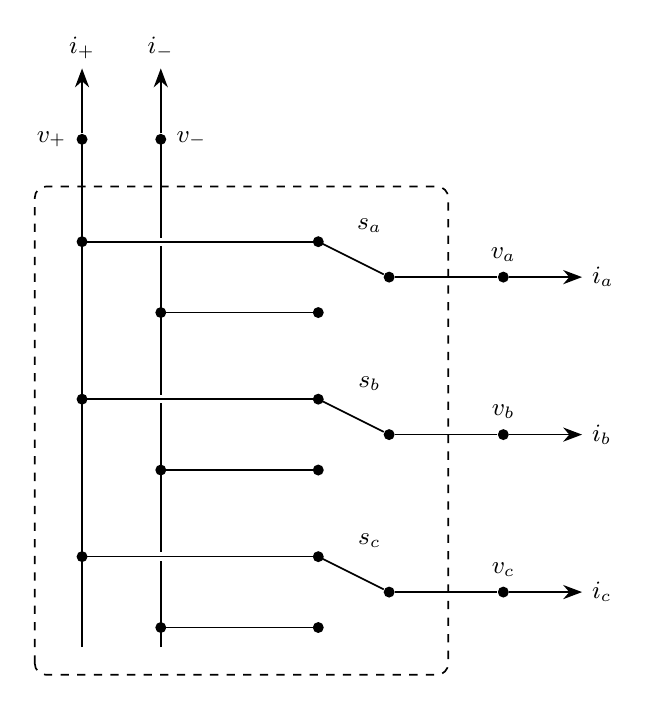
\begin{tikzpicture}[emt diagram]

% Common DC rails carry the aggregate current of the three depicted legs.
\draw[line] (-1,-2.7) -- (-1,3.75);
\draw[line] (0,-2.7) -- (0,3.75);
\node[signal, label={[sig]left:$v_+$}] (dcplus) at (-1,3.75) {};
\node[signal, label={[sig]right:$v_-$}] (dcminus) at (0,3.75) {};
\draw[->, line] (dcplus) -- ++(0,0.9) node[sig, above] {$i_+$};
\draw[->, line] (dcminus) -- ++(0,0.9) node[sig, above] {$i_-$};

% Representative a, b, c contacts share both rails.
% The upper position is drawn; the caption defines the smooth interpolation.
\foreach \y/\n in {\legrow/a,0/b,-\legrow/c} {
    \draw[wire jump] (-1,\y+0.45) -- (2,\y+0.45);
    \draw[line] (0,\y-0.45) -- (2,\y-0.45);
    \node[signal] at (-1,\y+0.45) {};
    \node[signal] at (0,\y-0.45) {};
    \node[signal] at (2,\y+0.45) {};
    \node[signal] at (2,\y-0.45) {};
    \node[signal] (ac\n) at (2.9,\y) {};
    \draw[line] (ac\n) -- (2,\y+0.45);
    \node[sig] at (2.65,\y+0.65) {$s_\n$};

    \node[signal, label={[sig]above:$v_\n$}] (v\n) at (4.35,\y) {};
    \draw[line] (ac\n) -- (v\n);
    \draw[->, line] (v\n) -- ++(1.0,0) node[sig, right] {$i_\n$};
}
% Electrical terminals remain outside the physical model enclosure.
\draw[enclosure] (-1.6,-3.05) rectangle (3.65,3.15);

\end{tikzpicture}
\end{document}
